% !TeX spellcheck = en_GB
% %%% ***************** CHAPTER INTRODUCTION ***************** %%%
\chapter{Introduction}
\label{ch:intro}
\textcolor{red}{\textbf{The overleaf file from the Introduction is here:} \\ \url{https://www.overleaf.com/13946064tcvpbpwjzjnk}}

%%%%%%%%% INTRODUCTION %%%%%%%%%%%%%%
During Christmas 2016 a storm impinged on the west coast of Norway. The storm, called 'Urd' was according to \cite{olsen_ekstremvaerrapport._2017} associated with strong winds and high precipitation amounts. The midwind along the coast of Western Norway had hurricane strength (observed: \SIrange{40}{55}{\mPs}). In South and Eastern Norway west to north-west winds between \SIrange{25}{40}{\mPs} were measured. At the Haukeliseter measurement site, \SI{136.4}{\milli\metre} of precipitation were monitored during \SIrange{21}{27}{\dec}.
This event was just above the limit of been called an extreme weather. Storms of this kind are expected to occur on average every five years \citep{olsen_ekstremvaerrapport._2017}. \\ 
The financial costs associated with 'Urd' are estimated to about 180 million Norwegian kroner.
'Urd' led to major traffic problems for cars, trains, ferries and air planes. Most mountain crossings were kept closed during Christmas 2016. 
In addition, there was a power breakout of around 70.000 households and 40 emergency power stations failed during the extreme weather. 
\\
This extreme weather, might not have lead to the same damages as some of the extreme weather events of recent years. But since people are affected by extreme weather (\Cref{fig:news}) it is important to predict storms, associated precipitation and wind as accurately as possible. Having accurate observations, will lead to better performing models which rely on observations. \textcolor{red}{include a reference here}
%%% images from Twitter and news %%%%%%%%%%%%%%%%%%%%%%%%%%%%%%%%%%%%%
% !TeX spellcheck = en_GB
\begin{figure}[t!]
	\centering
	\begin{subfigure}[b]{0.49\textwidth}
		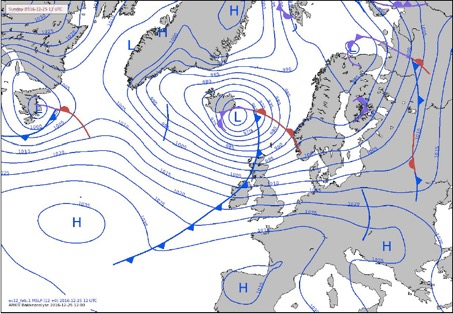
\includegraphics[width=\textwidth]{./fig_introduction/Ana_2512_12UTC.jpg}
		\caption{}\label{fig:ana_YR}
	\end{subfigure}
\hfill
	\begin{subfigure}[b]{0.49\textwidth}
		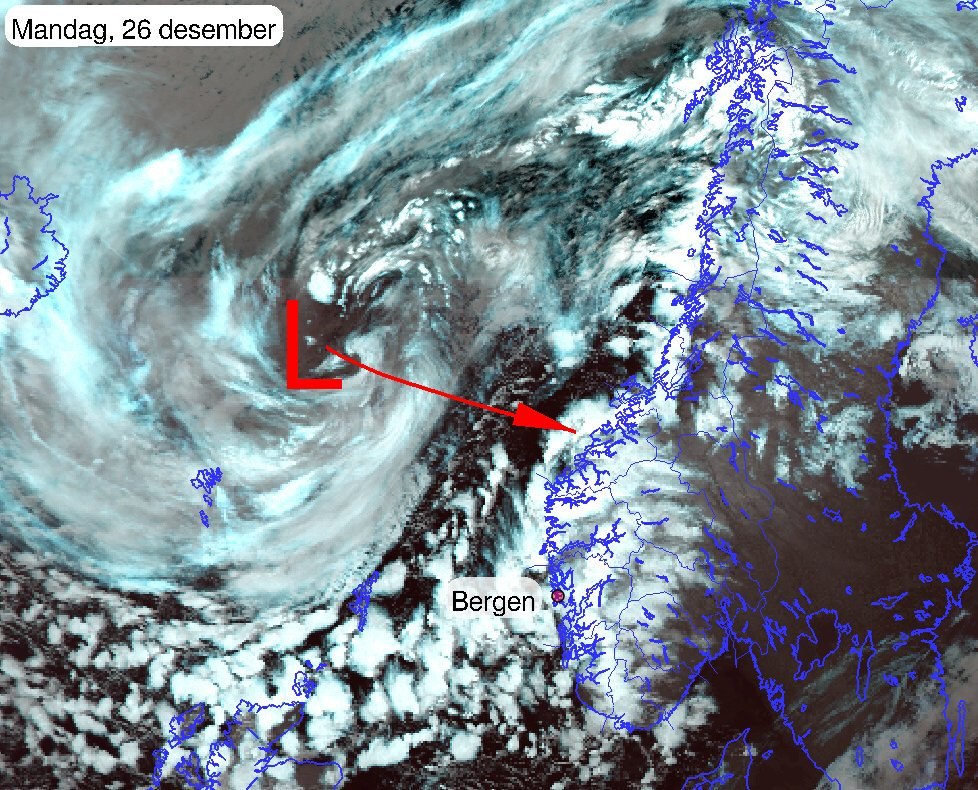
\includegraphics[trim={0cm 3.8cm 0cm 0cm},clip, width=\textwidth]{./fig_introduction/Twitter_26122016_0934AM.jpeg}
		\caption{}\label{fig:meteorologene_2612}	
	\end{subfigure}
	\begin{subfigure}[b]{0.49\textwidth}
		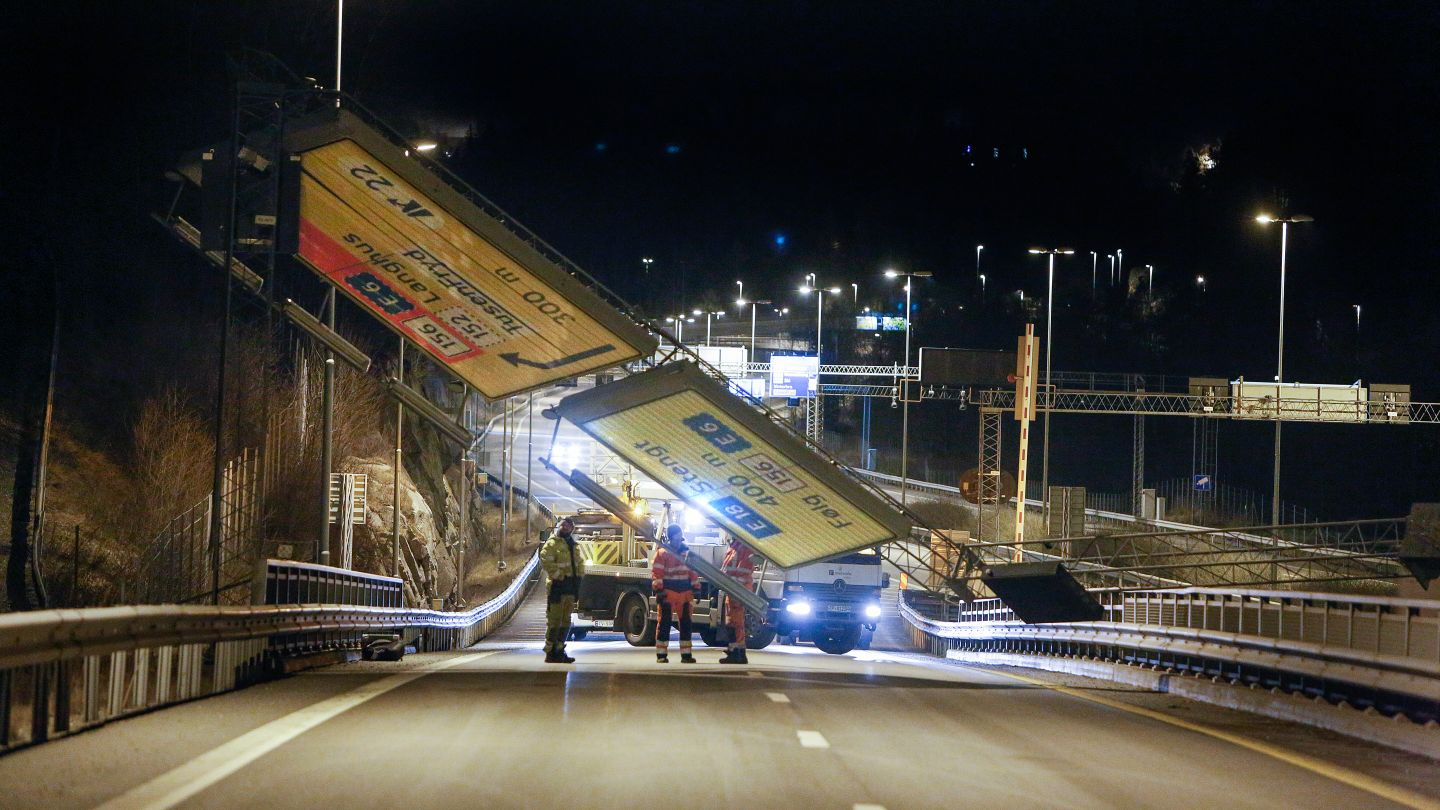
\includegraphics[width=\textwidth]{./fig_introduction/street_sign_2512.jpg}
		\caption{}\label{fig:street_sign}
	\end{subfigure}
\hfill
	\begin{subfigure}[b]{0.49\textwidth}
		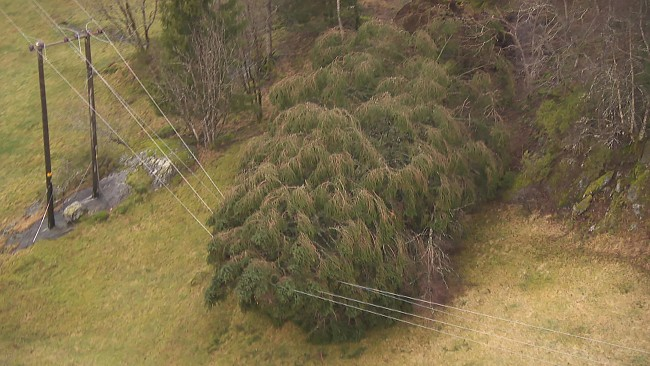
\includegraphics[width=\textwidth]{./fig_introduction/tree_nrk_2812.jpg}
		\caption{}\label{fig:tree_elec}
	\end{subfigure}
\caption{Weather situation during the extreme Christmas storm and impact on the infrastructure. In \protect\subref{fig:ana_YR}: Weather situation Sunday \SI{25}{\dec} at \SI{12}{\UTC} from the extreme weather report on Urd \citep{olsen_ekstremvaerrapport._2017}.
	\protect\subref{fig:meteorologene_2612}: Tweet from \cite{meteorologene_her_2016} on \SI{26}{\dec} at 9:34 am: Here comes \#Urd! The low pressure centre will hit M{\o}re og Romsdal, but the strongest wind comes south of Stad. \#S{\o}rNorge.
    \protect\subref{fig:street_sign} and \protect\subref{fig:tree_elec} show the consequences related to the high wind speeds during Christmas 2016.
	\protect\subref{fig:street_sign}: This traffic sign, ten meter long and four meter high was blown down during the storm, \citep{ruud_tonn_2016}.
	\protect\subref{fig:tree_elec}: Trouble maker: The extreme weather during Christmas created problems for the local infrastructure. \num{80.000} households were without electricity during the storm, \citep{farestveit_80.000_2016}.} \label{fig:news}
\end{figure}
%%%%%%%%%%%%%%%%%%%%%%%%%%%%%%%%%%%%%%%%%%%%%%%%%%%%%%%%%%%%%%%%%%%%%%%%%%
\newline
\noindent
\Cref{fig:news} shows that precipitation and strong winds can influence in certain ways the infrastructure. To predict and measure snowfall accumulation as accurately as possible is important since snowfall has impact on avalanches, freshwater release into water systems in spring, and extra economical expenses for local infrastructure as well as climatological effects. \\
\cite{joos_influence_2012} investigated the influence of microphysical processes on potential vorticity development in warm conveyor belts (WCB). They demonstrated the complex interaction between the small-scale microphyiscal processes and the large-scale flow in WCB. 
For the understanding of numerical simulations of storm developments it is important to know vertical precipitation profiles and their position within the synoptic vorticity environment. It is therefore crucial to study the vertical structure of different synoptic storms and  predict as accurately as possible.\\
% 
Since November 2016, the Meteorological Cooperation on Operational Numerical Weather Prediction (MetCoOP) Ensemble Prediction forecast (MEPS) is operational at the Meteorological Institute of Norway (Met-Norway). The study by \cite{muller_arome-metcoop:_2017} shows that the AROME-MetCoOp, a version of the Mèteo-France Applications of Research to Operations at Mesoscale, performs well for certain meteorological phenomena. \\
Microphysical processes in weather models are still not well understood and therefore are mostly parametrised \citep{muller_arome-metcoop:_2017}. Furthermore, high latitude regions are not well represented in meteorological models. Indeed a comparison between the MEPS data fit the observations for December 2016 but uncertainties are still present for this time period. 
\\
Some satellites, such as CloudSat have been equipped with radar to estimate snowfall rates and vertical profiles of precipitation. CloudSat is one of the satellites orbiting in the A-Train formation and measures the vertical structure of cloud systems \citep{stephens_cloudsat_2002}. 
\\
Studies of \cite{kulie_utilizing_2009} showed that the Cloud Profiling Radar (CPR), mounted on the CloudSat, can be used to estimate global distributions of snowfall. They showed that different combinations of microphyiscal habits and fall speed can lead to the same results of reflectivity and therefore to the same amount of snowfall rate.
Methods like optimal estimation retrieval were established to reduce the non-uniqueness. Where ground observations are used to estimate vertical profiles of precipitation.\\
The improvement of the CloudSat retrieval is helpful to show that climate models over estimate present-day Antarctic snowfall \citep{palerme_evaluation_2017}. \citet{norin_intercomparison_2015} presented a good agreement between the ground-based snowfall measurements and satellite observations. 

%%%%%%%%%%%%%%%%%%%%%%%%%%%%%%%%%%%%%%%%%%%%%%%%%%%%%%%%%%%%%%%%%%%%%%%%%%
%%%%%%%%%%%%%%%%%%%%%%%%%%%%%%%%%%%%%%%%%%%%%%%%%%%%%%%%%%%%%%%%%%%%%%%%%%
%%%%%%%%% HAUKELISETER SITE %%%%%%%%%%%%%%
\section{Measurement site - Haukeliseter}
\label{sec:site}
%%% images measurement site %%%%%%%%%%%%%%%%%%%%%%%%%%%%%%%%%%%%%
% !TeX spellcheck = en_GB
\begin{figure}[t]
	\centering
    \begin{subfigure}[b]{0.49\textwidth}
    	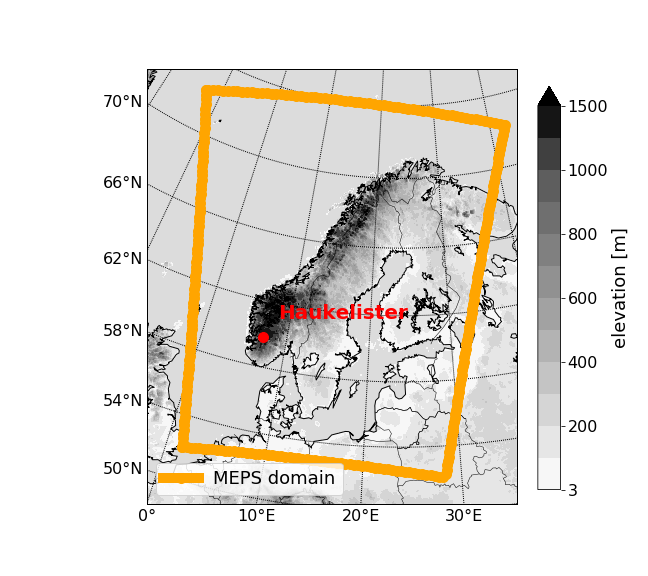
\includegraphics[trim={2.75cm 1.8cm 4.4cm 2.3cm},clip,
        width=\textwidth]{./fig_Norway/Norway_MEPS}
        \caption{}\label{fig:site:Norway}
    \end{subfigure}
 %%%%% zoomed in map
    \begin{subfigure}[b]{0.49\textwidth}
    	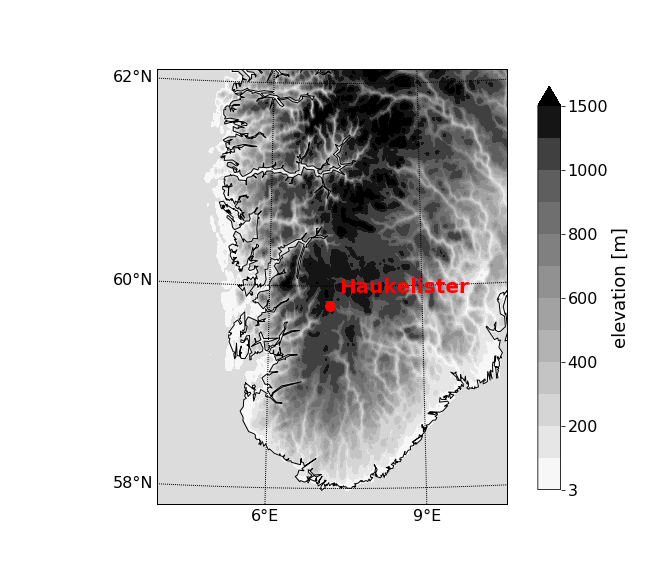
\includegraphics[trim={2.75cm 1.8cm .65cm 2.3cm},clip,
        width=\textwidth]{./fig_Norway/South_Norway}
    	\caption{}\label{fig:site:Nzoom}
    \end{subfigure}
   	\caption{Elevation map of Northern Europe and South Norway, \subref{fig:site:Norway}, \subref{fig:site:Nzoom} respectively. Red dot indicates the location Haukeliseter and the orange square in \subref{fig:site:Norway} indicates the model domain of MEPS. Elevation according to the shading.} \label{fig:site}
\end{figure}
%%%%%%%%%%%%%%%%%%%%%%%%%%%%%%%%%%%%%%%%%%%%%%%%%%%%%%%%%%%%%%%%%%%%%%%%%%
Haukeliseter, shown in \Cref{fig:site} is a mountain plateau \SI{991}{\m} above sea level, located in the Norwegian county 'Telemark' (\ang{59.8}\,N, \ang{7.2}\,E). The station measures precipitation, temperature, snow depth and wind. It has served as a measurement site for snow accumulation since the winter of 2010/2011 \citep{wolff_new_2010, wolff_measurements_2013, wolff_derivation_2015}. 
\\
In a study by \cite{wolff_derivation_2015} the wind-induced under-catch of solid precipitation is determined. Dependent on the kind of precipitation the wind plays different roles in the amount of accumulation. For temperatures below \SI{-2}{\celsius} the wind speed influences the falling snow. Where less precipitation can be observed at higher wind speeds or more precipitation can be measured if too much is blown into the gauge. The catch ratio between the standard Geonor precipitation gauge and the DF-Geonor shows, that only \SI{80}{\percent} of solid precipitation are observed at wind speeds of \SI{2}{\mPs} and only \SI{40}{\percent} at \SI{5}{\mPs}, \cite[Figure 5 in][]{wolff_derivation_2015}. The double fence gauge is more accurate than the single fence and is used as the reference gauge.
%\textcolor{red}{Steve: Should make some reference here to the vertical profile of observations needed to evaluate MEPS.  Me: What exactly does he mean?}. 
Nevertheless, this shows the need of a combination of ground based observations together with an optimal estimation retrieval to verify the accuracy of MEPS. \cite{wolff_derivation_2015} introduced an adjustment function for the Geonor double fence, so that different precipitation under certain wind speeds are presented correctly and can be used as confidential data. 

%%%%%%%%%%%%%%%%%%%%%%%%%%%%%%%%%%%%%%%%%%%%%%%%%%%%%%%%%%%%%%%%%%%%%%%%%%
%%%%%%%%%%%%%%%%%%%%%%%%%%%%%%%%%%%%%%%%%%%%%%%%%%%%%%%%%%%%%%%%%%%%%%%%%%
%%%%%%%%% DECEMBER OBSERVATIONS FROM WEATHERMAST %%%%%%%%%%%%%%
\section{Observations in December}
The general climate at Haukeliseter can be defined with the updated K\"oppen-Geiger climate types presented in \cite{peel_updated_2007}. Figure 8 in \cite{peel_updated_2007} shows, that Haukeliseter may lay in a transition zone and can be categorized as  ET, a polar tundra climate type (hottest month temperature T$_{hot}\ge$ \SI{0}{\celsius}) or Dfc, a cold climate without dry season and cold summers. 
\\
Haukeliseter presents a typical Norwegian climate condition. At the measurement site, frequent snow events combined with high wind speeds are observed during a six to seven month winter period. In addition a snow amount of about \SIrange{2}{3}{\m} can be expected, where \SI{50}{\percent} of the yearly precipitation is solid \citep{wolff_new_2010, wolff_measurements_2013, wolff_derivation_2015}. \\
The mean wind direction for solid precipitation is from the west with maximum wind speeds above \SI{15}{\mPs}, observed during a 10 year winter period at a nearby station \citep{wolff_new_2010, wolff_derivation_2015}. 
%%% images December observation %%%%%%%%%%%%%%%%%%%%%%%%%%%%%%%%%%%%%
% !TeX spellcheck = en_GB
\begin{figure}[t]
	\centering
    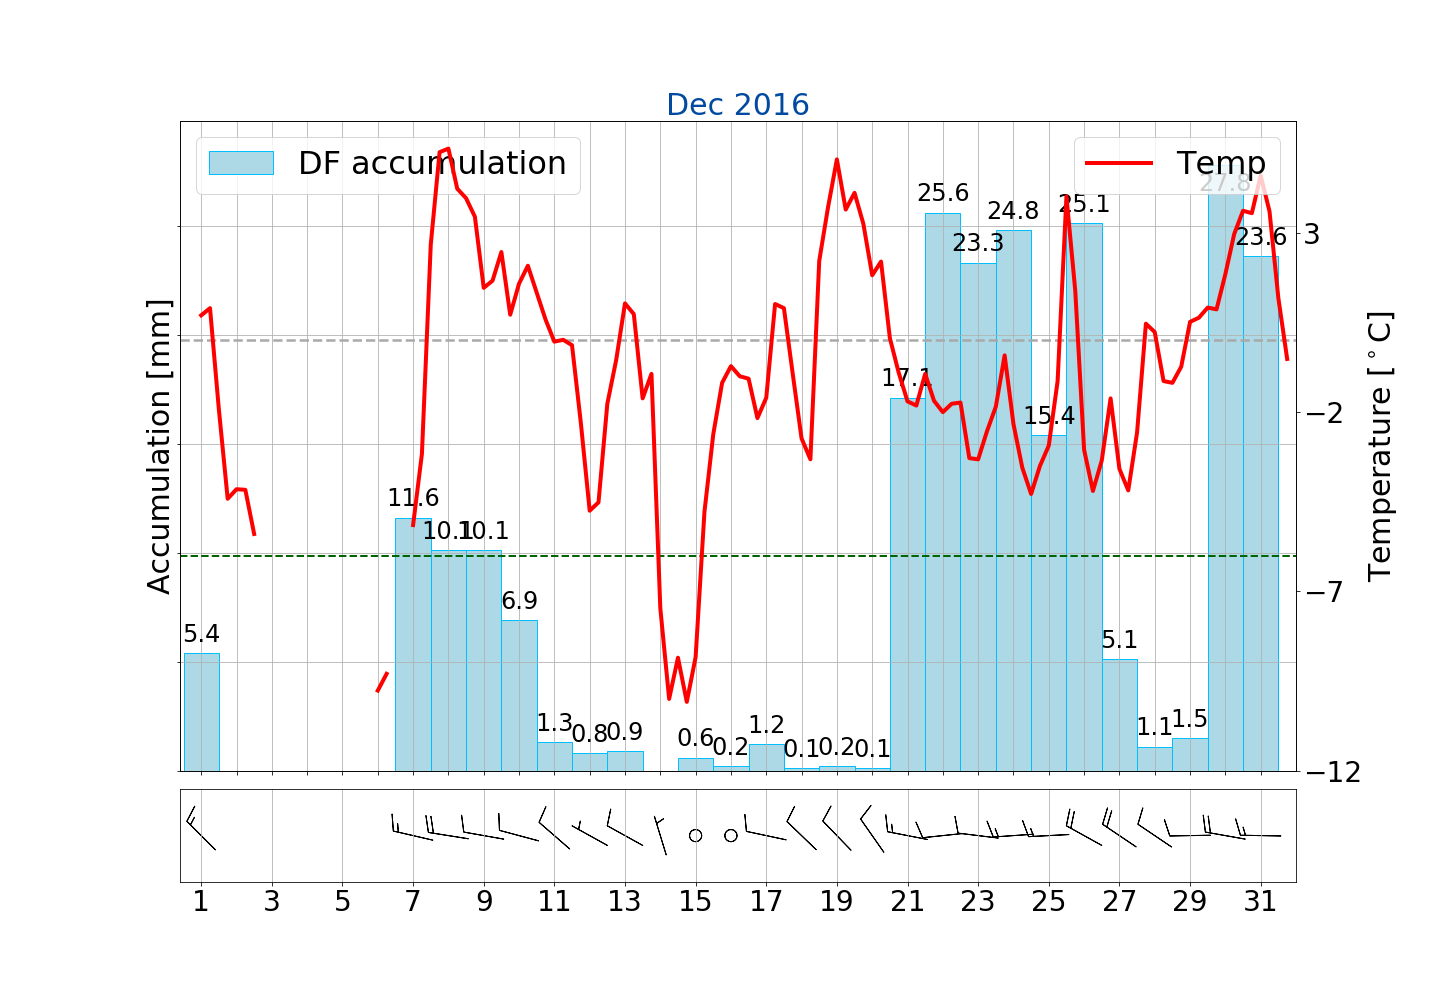
\includegraphics[trim={4.cm 3.3cm 1.5cm 3.cm},clip,
        width=0.8\textwidth]{./fig_weathermast/T_P_U_201612}
        \caption{Observations at Haukeliseter weather mast for December 2016. Daily accumulation [\SI{}{\mm}] in light blue, mean temperature every six hours (red, [\SI{}{\celsius}]), and daily maximum wind as barbs [\SI{}{\mPs}]. Gray dashed line indicates the freezing temperature. The monthly normal value is green dashed (\SI{-6.0}{\celsius}), the values are taken from \cite{eklima_norwegian_2016}. Note, that no data was available from \SIlist{2;6}{\dec}} \label{fig:DecObs}
\end{figure}
%%%%%%%%%%%%%%%%%%%%%%%%%%%%%%%%%%%%%%%%%%%%%%%%%%%%%%%%%%%%%%%%%%%%%%%%%%
\noindent As seen in \Cref{fig:DecObs} is the average December temperature \SI{-6}{\celsius} (30-yr period \numrange{1961}{1990}, value taken from \cite{eklima_norwegian_2016}). 
% mean temperature in Dec was -1.1°C, climate = -6 --> dT = 4.9°C
December 2016 was warmer with an anomaly of +\SI{4.9}{\kelvin} above the climate mean. 
% total precipitation in Dec is 239.9mm, climate = 85mm --> dRR = 154.9
In 2016, the precipitation was \SI{200}{\percent} more than the climate mean. \textcolor{red}{yr.no says something different. According to them was it only \SI{76}{\percent}} 
% total precipitation during 21.-27.12. is 136.4 mm, total is 239.9mm --> 56.9%
The precipitation observed in the time period \SIrange{21}{27}{\dec} where \SI{56.9}{\percent} of the total accumulation in December 2016. Furthermore, a maximum wind of \SI{22.3}{\mPs} was observed in this period, which can be associated to a slight storm.

%%%%%%%%%%%%%%%%%%%%%%%%%%%%%%%%%%%%%%%%%%%%%%%%%%%%%%%%%%%%%%%%%%%%%%%%%%
%%%%%%%%%%%%%%%%%%%%%%%%%%%%%%%%%%%%%%%%%%%%%%%%%%%%%%%%%%%%%%%%%%%%%%%%%%
%%%%%%%%% FIRST RESULTS MEPS, DOUBLE FENCE %%%%%%%%%%%%%%
\section{Preliminary MEPS and observation results}
\label{sec:PrelimMEPS}
As MEPS is operational since November 2016 one can compare the ensemble forecast model output with observations from the double fence at Haukeliseter. This will later on be compared to the vertical optimal snowfall retrieval estimates. 

%%% first results MEPS and DoubleFence %%%%%%%%%%%%%%%%%%%%%%%%%%%%%%%%%%%%%
% !TeX spellcheck = en_GB
\begin{figure}[t]
	\centering
%%%%%% 20/12
    \begin{subfigure}[b]{0.49\textwidth}
        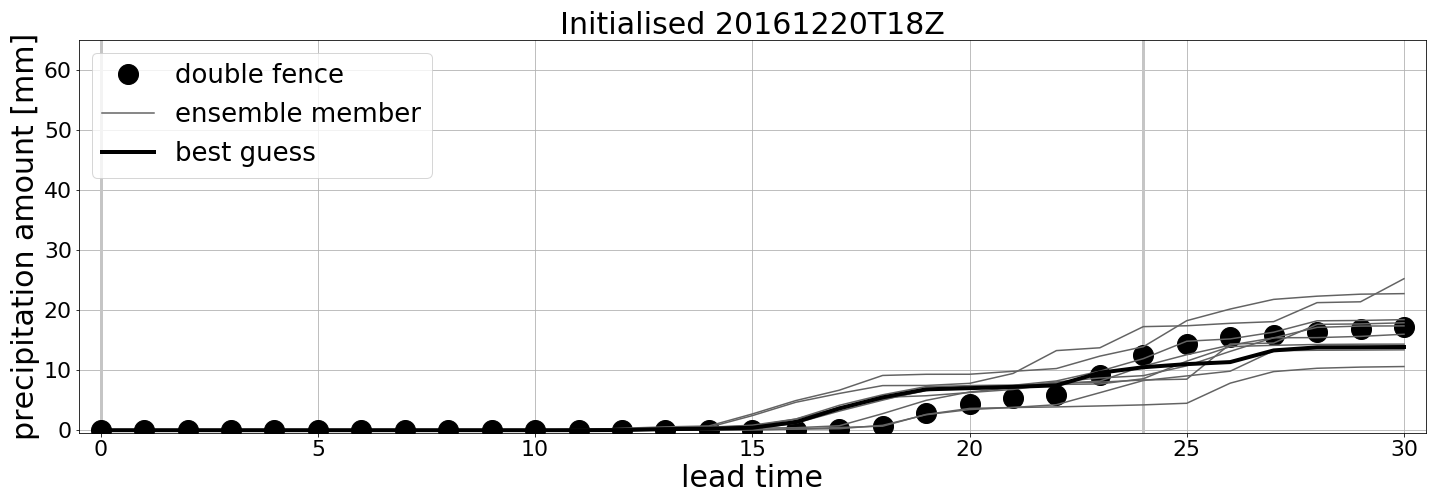
\includegraphics[
        width=\textwidth]{./fig_MEPS_sfc/20161220_18}
        \caption{}\label{fig:acc20}
        %\label{fig:DT2100}
    \end{subfigure}
    \hfill
%%%%%% 21/12
    \begin{subfigure}[b]{0.49\textwidth}
        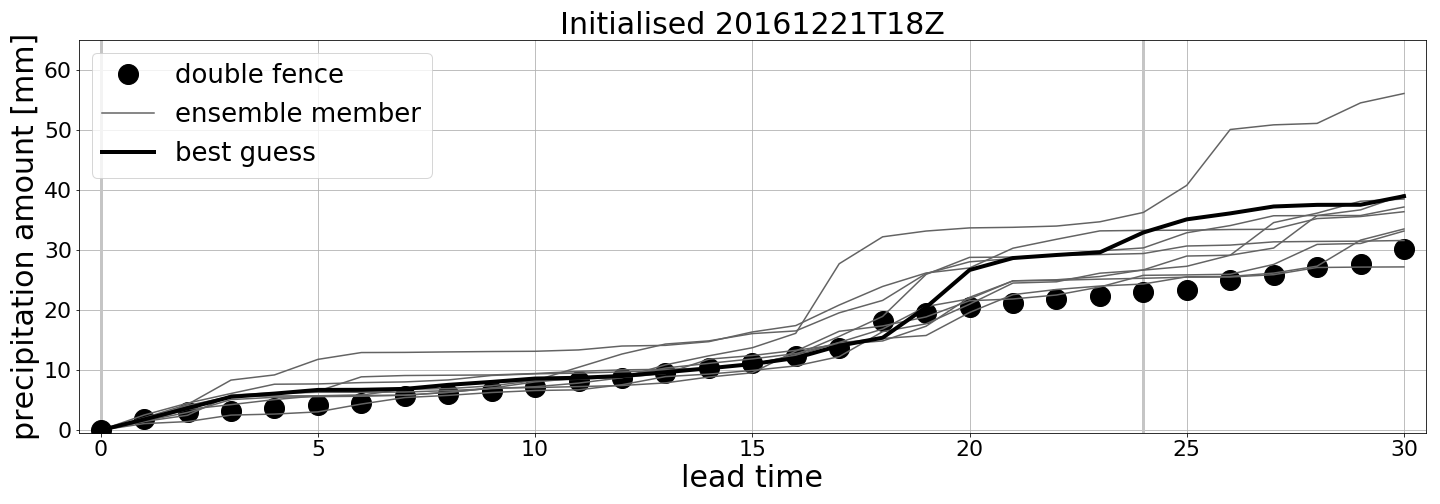
\includegraphics[
        width=\textwidth]{./fig_MEPS_sfc/20161221_18}
        \caption{}\label{fig:acc21}
    \end{subfigure}
%%%%%% 22/12
    \begin{subfigure}[b]{0.49\textwidth}
        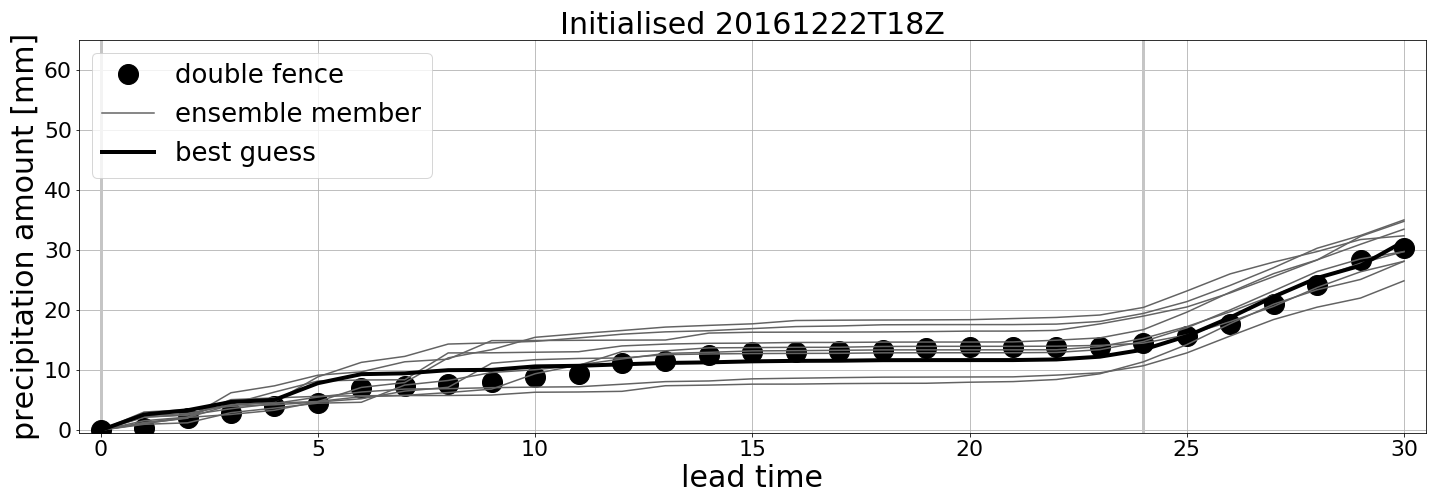
\includegraphics[
        width=\textwidth]{./fig_MEPS_sfc/20161222_18}
        \caption{}\label{fig:acc22}
    \end{subfigure}
    \hfill
%%%%%% 23/12
    \begin{subfigure}[b]{0.49\textwidth}
        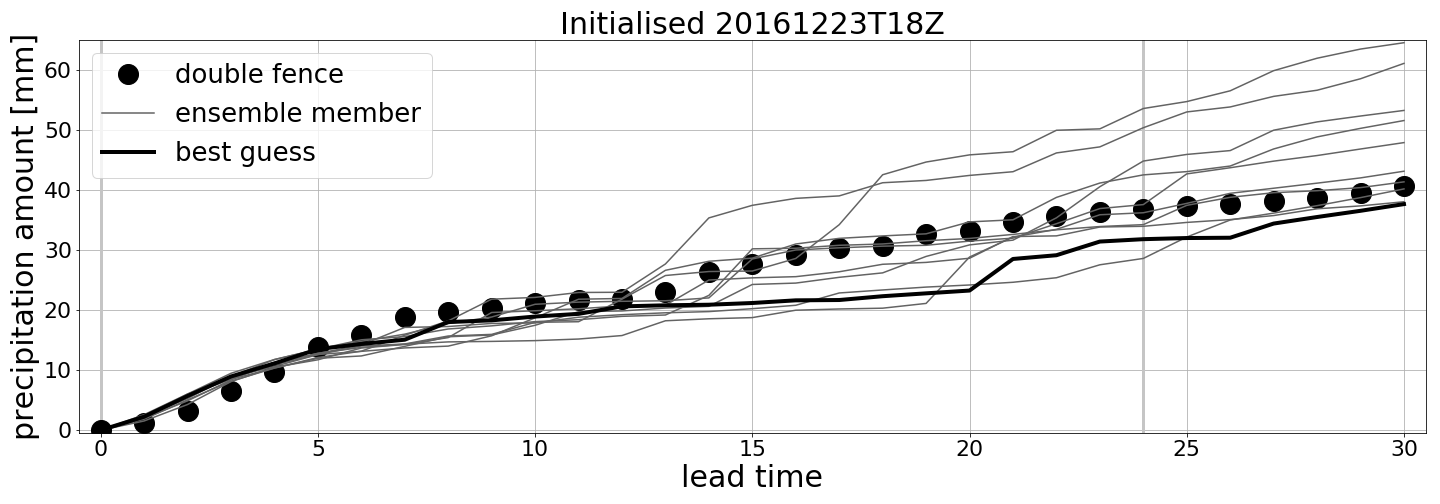
\includegraphics[
        width=\textwidth]{./fig_MEPS_sfc/20161223_18}
        \caption{}\label{fig:acc23}
    \end{subfigure}
%%%%%% 24/12
    \begin{subfigure}[b]{0.49\textwidth}
        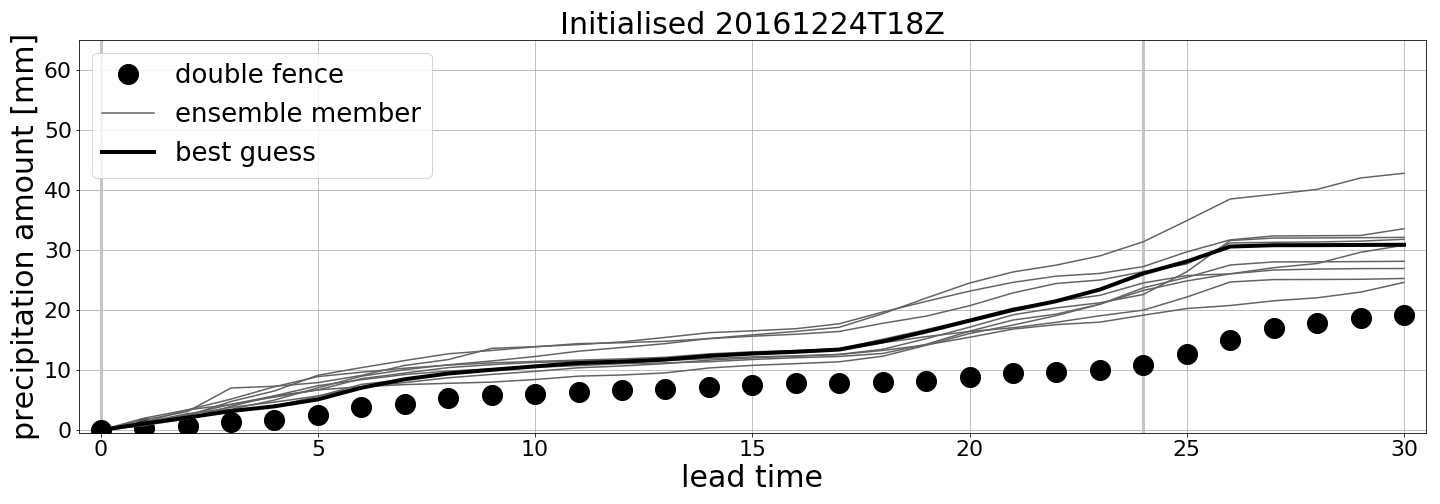
\includegraphics[
        width=\textwidth]{./fig_MEPS_sfc/20161224_18}
        \caption{}\label{fig:acc24}
    \end{subfigure}
    \hfill
%%%%%% 25/12
    \begin{subfigure}[b]{0.49\textwidth}
        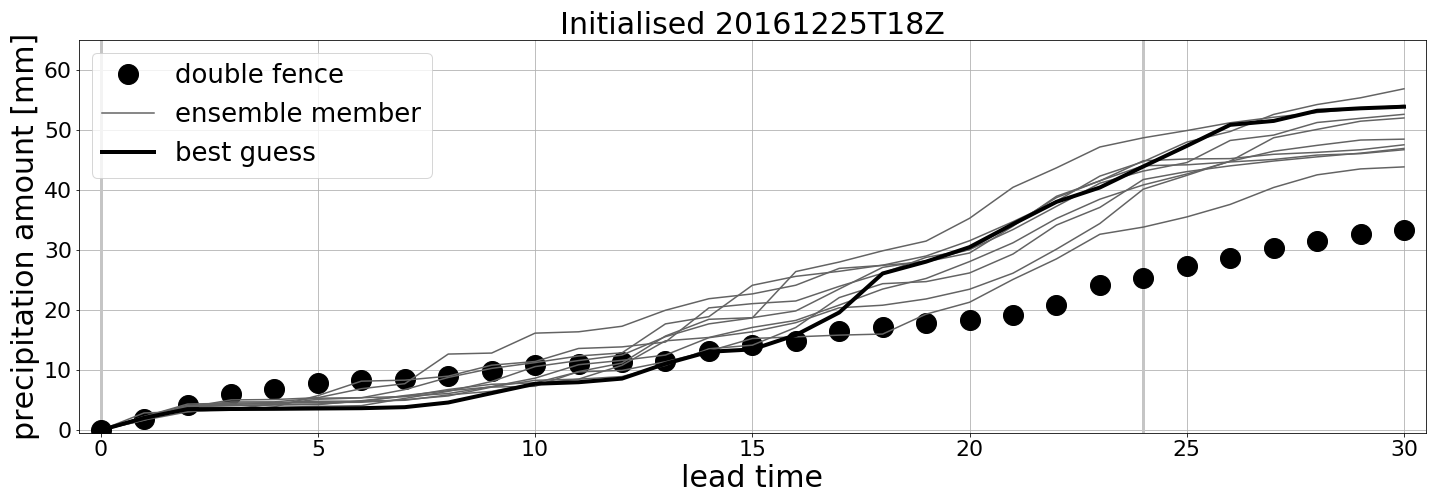
\includegraphics[
        width=\textwidth]{./fig_MEPS_sfc/20161225_18}
        \caption{}\label{fig:acc25}
    \end{subfigure}
    \caption{Accumulation of precipitation at Haukeliseter. Initalisation of MEPS at \SI{18}{\UTC}. Ensemble member as line in grey and the control in black. Dots indicate the hourly accumulation observed at the double fence, \citep{eklima_norwegian_2016}. \textcolor{red}{Do you think I have to make something bigger??? Font size etc? Or use one page only for the figures and have them underneath each other?} } \label{fig:acc20_25}
\end{figure}
%%%%%%%%%%%%%%%%%%%%%%%%%%%%%%%%%%%%%%%%%%%%%%%%%%%%%%%%%%%%%%%%%%%%%%%%%%
\noindent
During Christmas 2016 a storm approached the Haukeliseter site, which resulted in precipitation in form of liquid and solid.
\Cref{fig:acc20_25} shows the preliminary comparison between the MEPS ensemble member forecasts as well as the snowfall accumulation measured by the double fence at Haukeliseter. The double fence data is noisy and therefore, a filtered dataset is accessed from \cite{eklima_norwegian_2016}.   
\\
Each MEPS cycle is initialized at \SI{18}{\UTC} for the respective day.
Grey lines in \Cref{fig:acc20_25} show the nine perturbed ensemble members of MEPS. Where the black line reflects the control run, and the dots accumulation by the double fence.
\\
During the first few days the ensemble outputs cover the amount of snow good in comparison to the double fence observations.
The spread of the ensemble members around the control run fits as well to the observations for this time period. But, for an initialisation on the \SI{24}{\dec}, \SI{18}{\UTC} one can see that  MEPS over estimates the amount of snow accumulation. It is even more pronounced with the initialisation on the \SI{25}{\dec}, \SI{18}{\UTC} (compare \Cref{fig:acc25}). 
\\
This can have different reasons. One of them can be that the large scale weather situation was more predictable for the first four days (\Cref{fig:acc20,fig:acc21,fig:acc22,fig:acc23}). 
According to \cite{muller_arome-metcoop:_2017} are strong precipitation events better predicted with MEPS than ECMWF (European Centre for Medium-Range Weather Forecasts). On the other side, \cite{muller_arome-metcoop:_2017} states, that an overestimation appears, where the precipitation event (\SI{12}{\hour} accumulation) is less than \SI{10}{\mm}. This is not the case for the time period \SIrange{21}{26}{\dec} (compare \Cref{fig:DecObs}), where the daily precipitation exceed \SI{10}{\mm} every day. The question arises why MEPS covers the high amount of snow accumulation on the \SI{24}{\dec} but forecasts \SI{24}{\hour} prior to \SIlist{25;26}{\dec} are not covering the predicted amount of accumulation!